\documentclass[../../../include/open-logic-section]{subfiles}

\begin{document}

\olfileid{sth}{ordinals}{idea}
\olsection{ترتیبی عدد دا عام خیال}

قدرتی عدداں نوں اوہناں دی عام ترتیب وچ ویکھو:
\begin{center}
	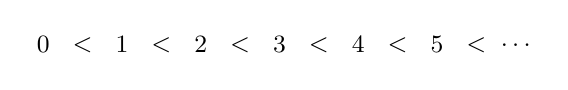
\begin{tikzpicture}
	\foreach \x/\xtext in {0, 1, 2, 3, 4, 5}
	{
		\node (\x a) at (\x, 1) {\small{$\x$}};
		\node (\x a) at (\x.5, 1) {\small{$<$}};
	}
	\node (ldots) at (6, 1) {\small{$\ldots$}};
	\end{tikzpicture}
\end{center}
فنی بولی وچ اینوں $\omega$ والی لڑی آکھدے آں۔ واقعی ایہ عام ترتیب سیٹاں
دی درجہ بندی دے مرحلیاں دی مُڈھلی بناوٹ وچ وی دِسدی اے۔ پر ہُن منّ لو اسیں
$0$ نوں لڑی دے آخری سرے اُتے لے جائیے، تاں جو اوہ سارے ہور عدداں توں
پچھوں آوے:
\begin{center}
	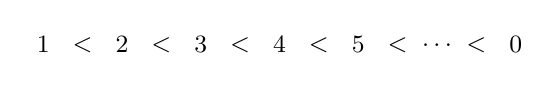
\begin{tikzpicture}
	\foreach \x/\xtext in {1, 2, 3, 4, 5}
	{
		\node (\x a) at (\x, 1) {\small{$\x$}};
		\node (\x a) at (\x.5, 1) {\small{$<$}};
	}
	\node (ldots) at (6, 1) {\small{$\ldots$}};
	\node (bea) at (6.5, 1) {\small{$<$}};
	\node (noa) at (7, 1) {\small{$0$}};
	\end{tikzpicture}
\end{center}
ایتھے شےواں اوہو نیں، پر اوہناں دی ترتیب بنیادی طور اُتے وکھری اے۔
پہلی ترتیب دا کوئی آخری عنصر نہیں سی، نویں ترتیب دا اے۔ واقعی نویں
ترتیب وچ شےواں دی اک $\omega$ والی لڑی ($1, 2, 3, 4, 5, \ldots$) اے
تے اوہدے پچھوں اک ہور شے اے۔ ایہ $\omega+1$ والی لڑی ہووے گی۔

صرف ایہو شےواں ورت کے اسیں ہور وی کئی قسم دیاں ترتیباں بنا سکدے آں۔
مثلاً سارے جفت عدد (اوہناں دی قدرتی ترتیب وچ)، تے اوہناں توں پچھوں
سارے طاق عدد (اوہناں دی قدرتی ترتیب وچ) ویکھو:
\begin{center}
	\begin{tikzpicture}
	\node(a1) at (1,1) {\small{$0$}};
	\node(a2) at (1.5,1) {\small{$<$}};
	\node(a3) at (2,1) {\small{$2$}};
	\node(a4) at (2.5,1) {\small{$<$}};
	\node(a5) at (3,1) {\small{$4$}};
	\node(a6) at (3.5,1) {\small{$<$}};
	\node(dots) at (4,1) {\small{$\ldots$}};
	\node(aaoe) at (4.5,1) {\small{$<$}};
	\node(b1) at (5,1) {\small{$1$}};
	\node(b2) at (5.5,1) {\small{$<$}};
	\node(b3) at (6,1) {\small{$3$}};
	\node(b4) at (6.5,1) {\small{$<$}};
	\node(b5) at (7,1) {\small{$\ldots$}};
	\end{tikzpicture}
\end{center}
ایہ اک $\omega$ والی لڑی اے جیہدے پچھوں دوجی $\omega$ والی لڑی اے،
یعنی $\omega+\omega$ والی لڑی۔

اسیں اگے ودھ سکدے آں۔ پر سانوں \emph{ترتیباں} دی ایس گل بات نوں
سمجھن دا اک عام طریقہ چاہیدا اے۔

\end{document}
